\documentclass{sig-alternate-05-2015}
% Load basic packages
\usepackage{balance}  % to better equalize the last page
\usepackage{graphics} % for EPS, load graphicx instead 
\usepackage[T1]{fontenc}
\usepackage{txfonts}
\usepackage{mathptmx}
\usepackage[pdftex]{hyperref}
\usepackage{color}
\usepackage{booktabs}
\usepackage{textcomp}
\usepackage{xspace}
\usepackage{setspace}
\usepackage[textsize=tiny]{todonotes}
% Some optional stuff you might like/need.
\usepackage{microtype} % Improved Tracking and Kerning
% \usepackage[all]{hypcap}  % Fixes bug in hyperref caption linking
\usepackage{ccicons}  % Cite your images correctly!
% \usepackage[utf8]{inputenc} % for a UTF8 editor only
\usepackage{verbatim}
%Suppress Copyright box
\usepackage{etoolbox}
% \makeatletter
% \patchcmd{\maketitle}{\@copyrightspace}{}{}{}
% \makeatother
\makeatletter
\def\@copyrightspace{\relax}
\makeatother

\usepackage{relsize}
\usepackage{etoolbox}
\usepackage{lipsum}   % for filler text
\usepackage{setspace} % for \onehalfspacing and \singlespacing macros
\usepackage[normalem]{ulem}
\usepackage[sort,nocompress]{cite}
\AtBeginEnvironment{quote}{\singlespacing\small \vspace{-16pt}}
\AtEndEnvironment{quote}{\vspace{-6pt}}
%\def\plaintitle{Learning through play: Iterative query-seeking through partial query specification}
\def\plaintitle{Iterative query-seeking through partial query specification}
\def\plainauthor{Doris Jung-Lin Lee}
\def\emptyauthor{}
\def\plainkeywords{Data visualization, exploratory data analysis, visual query, scientific data.}
\def\plaingeneralterms{Documentation, Standardization}

% llt: Define a global style for URLs, rather that the default one
\makeatletter
\def\url@leostyle{%
  \@ifundefined{selectfont}{
    \def\UrlFont{\sf}
  }{
    \def\UrlFont{\small\bf\ttfamily}
  }}
\makeatother

\newenvironment{denselist}{
    \begin{list}{\small{$\bullet$}}%
    {\setlength{\itemsep}{0ex} \setlength{\topsep}{0ex}
    \setlength{\parsep}{0pt} \setlength{\itemindent}{0pt}
    \setlength{\leftmargin}{1.5em}
    \setlength{\partopsep}{0pt}}}%
    {\end{list}}

\newcommand{\squishlist}{
   \begin{list}{$\bullet$}
    { \setlength{\itemsep}{0pt}
      \setlength{\parsep}{2pt}
      \setlength{\topsep}{0pt}
      \setlength{\partopsep}{0pt}
      \leftmargin=25pt
\rightmargin=0pt
\labelsep=5pt
\labelwidth=10pt
\itemindent=0pt
\listparindent=0pt
\itemsep=\parsep
    }
}
\newcommand{\squishend}{\end{list}}

% use extensively to toggle between paper and TR
\newcommand{\eat}[1]{}
\newcommand{\papertext}[1]{#1}
\newcommand{\techreport}[1]{}


% de-facto paragraph format
\newcommand{\stitle}[1]{\noindent\textbf{#1}}

\urlstyle{leo}

\newcommand{\subsubsectionlong}[1]{

{\subsecfnt #1}

\vspace{-6pt}}

\newcommand{\subsectionlong}[1]{

{\secfnt #1}

\vspace{-6pt}}

% To make various LaTeX processors do the right thing with page size.
\def\pprw{8.5in}
\def\pprh{11in}
\special{papersize=\pprw,\pprh}
\setlength{\paperwidth}{\pprw}
\setlength{\paperheight}{\pprh}
\setlength{\pdfpagewidth}{\pprw}
\setlength{\pdfpageheight}{\pprh}

% Make sure hyperref comes last of your loaded packages, to give it a
% fighting chance of not being over-written, since its job is to
% redefine many LaTeX commands.
\definecolor{linkColor}{RGB}{6,125,233}
\hypersetup{%
  pdftitle={\plaintitle},
% Use \plainauthor for final version.
%  pdfauthor={\plainauthor},
  pdfauthor={\emptyauthor},
  pdfkeywords={\plainkeywords},
  bookmarksnumbered,
  pdfstartview={FitH},
  colorlinks,
  citecolor=black,
  filecolor=black,
  linkcolor=black,
  urlcolor=linkColor,
  breaklinks=true,
}

\begin{document}

% Copyright
% \setcopyright{acmcopyright}
%\setcopyright{acmlicensed}
%\setcopyright{rightsretained}
%\setcopyright{usgov}
%\setcopyright{usgovmixed}
%\setcopyright{cagov}
%\setcopyright{cagovmixed}

%
% --- Author Metadata here ---
%\CopyrightYear{2007} % Allows default copyright year (20XX) to be over-ridden - IF NEED BE.
%\crdata{0-12345-67-8/90/01}  % Allows default copyright data (0-89791-88-6/97/05) to be over-ridden - IF NEED BE.
% --- End of Author Metadata ---
\title{\plaintitle}
\author{\plainauthor}
\maketitle
% \begin{abstract}
% Abstract
% \end{abstract}
\section{Introduction}
Formulating ad-hoc database queries for exploratory data analysis is a challenging problem for analysts. %Prior work in query-by-example and query synthesis address this by inferring candidate queries based on input and output data examples and visual query construction through a specification interface. However, the more pressing challenge for both novice and expert analysts is often coming up with the right question to ask.
While many existing systems have been developed to make it easier to perform query specification in exploratory analysis\cite{Khoussainova2010,Nandi2013,Wu2013,Vartak2015,Abouzied2012,Jiang2015}, the more pressing challenge of how to help analysts come up with the right questions to ask is relatively unexplored. Most of these prior work have focussed on intent-to-query mapping mechanisms that assume users have a question in mind to begin with. Therefore, these work focuses on resolving the ``language barrier'' to help novices unfamiliar with SQL issue queries to the database. However, users often only have minimal or partial ideas on what types of data operations they would like to perform or the types of query they are interested in.  Moreover, while existing database query interface are capable of synthesizing SQL queries based on high-level specifications, the space of queries that could be issued with these interface are often limited by the set of form fields and interactions envisioned by tool-designers. A more natural mode of interaction is perhaps to specify the the known examples and relations of interest, albeit partial, to the system, and let the system infer what is best to show to the user.
\par To this end, we proposed a unifying query language that captures a wide spectrum of query input specificity, called partial query language (PQL). Unlike structured querying languages, which are monolithic and evaluates only upon exact specification, PQL is tolerant to the inherent ambiguity of user specification. PQL takes in an underspecified query during exploratory data analysis, the system suggests interesting relations or examples to query with or further actions. Based on the user's feedback on the seen output, the system updates the next set of recommendations. The goal of PQL is to simultaneously enable flexible querying as well as gain better understanding of the dataset to facilitate users to discover the interesting questions to ask.
% These underspecified query can include requests for overviews, uncertain attributes selections, or view suggestions within a range query. 

%\begin{figure}
%\centering
%\includegraphics[height=1in, width=1in]{fly}
%\caption{A sample black and white graphic
%that has been resized with the \texttt{includegraphics} command.}
%\end{figure}

% Contribution: 
% \begin{itemize}
% \item unifying model for inference
% \item vizRec that account for feedback (not based on logs)

% Our key idea is to make use of feedback to support partial queries. 
% IR relevance feedback
% idea that queries are hard to come up with, but it should be easy to rate something or say if it is relevant or not. 
% Dataplay has this with "want-in", "want-out example"
% \end{itemize}
% The first two are language features of PQL and the latter two requirements are related to the PQL engine. 
\begin{figure}[ht!]\label{system}
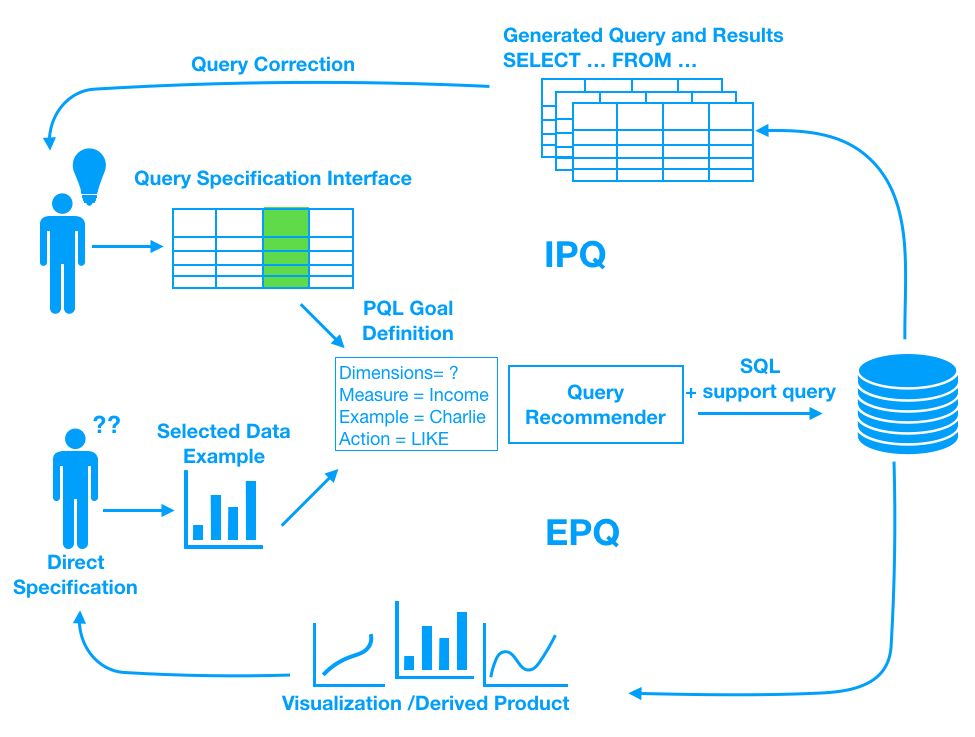
\includegraphics[width=\linewidth]{figures/system.png}
\caption{System architecture highlighting the relational and example partial query use cases. The users can move seamlessly across different query specification mechanisms to iteratively improve their query.}
\end{figure}
\section{Motivation \& Related Works}
\par Despite extensive work in database usability, there is an inevitable design trade-off between the query expressivity and interface usability\cite{Jagadish2007,Morton2014}. Given that there is no one size fit all interface for query specification for users of different expertise levels and workload, PQL is designed as a middle-layer between the interface and querying engine that can take in a wide spectrum of queries of different input types and degrees of specificity that could be potentially generated from different interfaces. Here, we list the potential query inputs in order of increasing specificity: 
\begin{itemize}
\item \textbf{Cold-start}: no supervision, only given dataset as input. (viz-summarization is a more supervised version of this where measure and group-by dimensions of interest are given.)
\item \textbf{Example-based partial queries (EPQ)}: EPQs takes in data examples based on what they have already seen and use this to jumpstart their query. 
%\par Given an EPQ, PQL infers and suggest potential explanations or queries based on the data the user provides as a query. 
%A crucial difference that separates our work and QBE is that the goal of EDPQ is to generate potential explanations or query recommendations rather than generating a query that will address a predefined question. As a result, EDPQ has a more relaxed set of constraints compared to typical scenario in the query synthesis problem, which leads to a larger search space potential queries that offer further opportunities for optimization.
\par Existing work in query-by-examples (QBE) asks users to provide I/O examples of the query to be synthesized\cite{Wang2017a,Wang2017}. However, if the user does not know what they are querying for, then they would not be able to come up with such an example. In addition, EPQ accepts a more easy-to-come-up-with input modalities such as visualization distributions or an existing singleton record as examples to query. The types of inputs could be largely classified in two categories: 1) Record querying: querying via non-aggregated set of tuples or visualizations as input (e.g. drag-and-drop in Zenvisage, smart drill down) or 2) Result querying: querying via transformed tuples (aggregation, top-k), often for offering explanations\cite{Chapman2009,Wu2013,Roy2015}.
%These example inputs to queries comes from the results of support queries. Support queries are queries that are non-essential in answering the queries, but provide auxcillary information that could help users jumpstart in their hypothesis generation. Examples of support queries includes requests to overview representatives, outliers, and other statistics, or generate different types of visualizations. These support queries can be either system generated (as part of suggestions and explainations) or defined by the user. 
\item \textbf{Relational partial queries (RPQ)}: RPQs follow the conventional approach to querying a database where a user starts with a pre-existing idea of what he is looking for based on what he has already seen or know. However, formulating SQL queries that maps user's high-level intentions to specific query statements is challenging. 
 %The way that analyst B approached the problem is an example of this. %For example, he may be trying to explore an attribute in more detail to test a hypothesis or he may be looking for examples of highly-performing young innovators. 
\par Recent work in natural language querying have tried to address this by parsing adjectives and quantifiers and asking the users for additional information to resolve the ambiguity through form-based interface if needed. Similar to form-based or visual query builders\cite{Abouzied2012}, these systems are often based on templated queries with limited expressiveness in their linguistic and conceptual coverage, which makes it difficult for expert users to express complex queries. SnipSuggest addresses this problem by recommending relevant snippets of SQL queries based on partial queries (user's partially typed input) via auto-complete\cite{Khoussainova2010}. However, their context-aware algorithm crucially depends on the existence of a query workload. 
%\par Instead of approaching this problem from the perspective of ambiguity resolution, we recognize that sometimes users themselves may not have a clear cut specification of what they are asking for. As a result, we introduce the EXPLORE operator and the special value ? to increase the tolerance of ambiguity inherently in the PQL language design, then the engine takes this partial specification decide what would be the best answers or suggestions to return as an output.
%\item relational querying: SnipSuggest, DataPlay, form-based or visual query builders (ZQL)
\item \textbf{Complete specification}: At the highest level of specification, there is SQL and direct manipulation interfaces that performs database operations based on complete specification.
\end{itemize}
%these two inter-related modes of data exploration, where data or bottom up approaches are initiated through data examples and framing comes from specifying distribution or relationships in a top-down manner.
\section{Usage Scenario}
\par A team of analyst is a given a dataset that consists of the reported income of individuals. They wanted to investigate whether there is any evidence of institutional bias on worker salaries. Given this large dataset with hundreds of attributes and records, they are unsure of where to start. The only thing they know is that they care about the Income column, so they specify this as the measure attribute of interest in PQL by brushing the Income column in yellow (Figure \ref{example} top). In this initial step, PQL tries to provide as much support information as it can by displaying a sample table of data records arranged in the order of increasing income, the attributes are displayed in the order of most to least importance, where importance is defined by how much the feature have an impact on the measure variable of interest. By convention, the primary key is always in the first column. These attribute-importance ranking techniques populates the most important relations that the users has to see in the first few visible columns.
\par Given this information, analyst A was still not able to infer anything about any particular column to ask a new question, but notices that Charlie has an incredibly low income compared to average. Using PQL specification interface, he uses the green paintbrush to highlight the record for Charlie and specifies the action to look for other records similar to Charlie. He notices that all of the returned records are all young children who work part-time jobs.
\begin{figure}[ht!]\label{example}
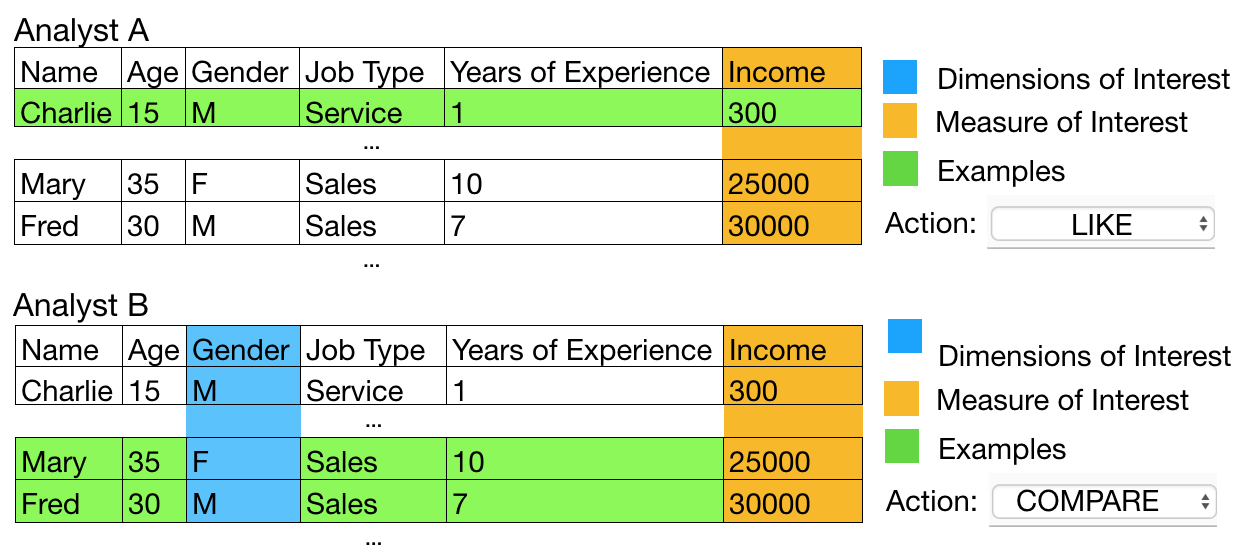
\includegraphics[width=\linewidth]{figures/example2.png}
\caption{One example of a potential interface that could be used for submitting PQL queries. Users can select examples or columns of interest. }
\end{figure}
\par Analyst B skims through the records and notices that despite Mary having more years of working experience than Fred, she is getting paid \$5000 less than him. He wants to find out whether employers are marginalizing the pay of certain individuals based on gender for the same job done. He colors the Gender column in yellow and the record of Mary and Fred in green, then specifies the ``COMPARE'' action (Figure \ref{example} bottom). Given this PQL specification consisting of a mix of records, dimensions and measure attributes, the example finding algorithm in PQL finds records that are similar to Fred AND Mary, while distinguishing these groups of records by gender. The results consist of two tables corresponding to males and females with similar credentials as Fred and Mary. Using the records and supporting overview statistics and histograms for the corresponding result-sets, analyst B finds that Gender is not a factor in determining Income and that the observed example was an anomaly and seeks for additional hypothesis that explains the difference between Mary and Fred.
%Given this hypothesis, he specifies a PQL query to find women who are in Sales and have similar years of experience as Mary and Fred. The PQL engine generates two support queries on this selected population to display the overview statistics and histograms of the selected subpopulation and its counterpart (i.e. men who are in Sales with similar years of experience).
\section{PQL Design}
%Reflecting the two ---, PQL supports these two corresponding types of queries:  
The language design of PQL is motivated by several desiderata:
\begin{enumerate}
	\item Tolerant to ambiguity : PQL must have a model of inference that can make inference with incomplete specification, since 1) partial queries can be used for jump-starting the exploration of under-developed hypothesis and 2) queries can be iteratively refined by the user as user gain more information about the data to update the model. 
  \item Model does not depend on a domain-specific query workload: Many existing systems makes use of information from query logs to provide ``typical workload'' query recommendations\cite{Morton2014,Kamat2016,Khoussainova2010}. However, the existence of such workloads is not commonly available outside of large enterprises or scientific collaboration setting. In addition, while PQL can be used for all stages of analysis, it is most beneficial to the users at the early-stages of data analysis. So if there is a pre-existing queries performed, it means that a detailed analysis had already been performed and the insights from that analysis (e.g. through documentations) should have given the analyst a better idea on what questions to ask next. Without the query workload, the model of inference must work with minimal user input and be updatable upon additional user input.
	\item Composability: PQL operators must be composable to increase the expressiveness of PQL in supporting a large class of ad-hoc queries, so that analysts are not constrained when exploring the types of questions they might want to ask.
	\item Supporting both records and relations as inputs : Given the prior work of how analyst make sense of their data\cite{Pirolli2005,Klein2006}, PQL must support both bottom-up example records and top-down relational specification of queries. As shown in the usage scenario, given the same data output, different analysts may have different interpretation and approach the same dataset and problem. %PQL enables analysts to seamlessly switch between the two modes of inquiry as shown in Figure \ref{architecture}.  %Popular theories in data sensemaking have suggested two different symbiotic modes of operations for understanding data. Pirolli and Card’s notional model describes information processing as an ``opportunistic mix'' between top-down (from theory to data) and bottom-up (from data to theory) tasks\cite{Pirolli2005}. Similarly, the Data/Frame theory suggests that the data analysis process is a closed-loop transition between an effort to recognize or construct a frame through data or defining connections amongst the seen data\cite{Klein2006}. 
	%\item Ability to suggest possible actions: The suggestion can come in two forms: 1) Given a partial query, suggest the possible queries that are \textit{simmilar in functionality} or 2) Given a data example or resultset, suggest possible next steps or actions that reflect \textit{simmilar data relationships}.
	%\item Model takes in feedback
	% \item Ability to generate explainations: Simmilarly explaination could be 1) by-example: data/record-level locality, or 2) by theory: membership or behaviour locality.
\end{enumerate}
PQL can be written in terms of action-operators and goal definitions. Goal definitions specifies the attributes and records that users are interested in. There are three types of goal definitions supported by PQL: 
\begin{itemize}
	\item Attribute-value of interest (e.g. GENDER= 'Female')
	\item Attribute of interest (e.g. GENDER=?): can either be a measure or dimension. Measure of interest have a special significance in the algorithm.
	%OBJECTIVE $M$ : Defining the measure value of interest during the analysis as M.
	\item Non-aggregated example records $\{r_1 ...r_n\}$: Point queries where all attribute-values are completely specified (e.g. Mary: GENDER=F, Age=35, ..., Income = 25k)
\end{itemize}
\begin{figure}[ht!]\label{nodeType}
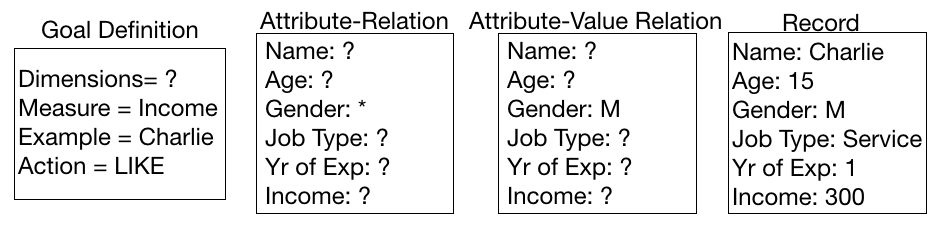
\includegraphics[width=\linewidth]{figures/nodeTypes.png}
\caption{An example PQL specification is shown on the left with ? denoting the underspecified values. The three types of goal definitions are shown in the right.}
\end{figure}
Any unspecified goal definitions is denoted with the special value ``?''. Action-operators can take a record ($r_i$) or relation ($A_i$) as inputs and outputs and performs some action. Action-operators can be decomposed as a set of goal definitions. Examples of action-operators includes:   
\begin{itemize}
  \item DISTINGUISH $r_i$: Find the distinguishing feature of $r_i$.
	\item EXPLORE $\{A_1 ...A_n\}$: Overview or Drill-down to attribute(s) of interest.
	\item EXPLAIN $r_i$: Tracing the lineage of $r_i$.
	\item LIKE $\{r_1 ...r_n\}$: Find records that are simmilar to $r_i$.
	\item COMPARE $\{r_1 ...r_n\}$: Compare why two or more records are different.
\end{itemize}
% \par Using the example table shown in Figure.\ref{edpq_example}, examples of EDPQ includes: 
% Given a queried record, 
% PQL engine generates \textit{support queries}.
%the ability to work with individual record-level examples and compare  
\section{Problem Formulation}
Described below are two approaches that I am currently exploring for the problem of query recommendation given a PQL specification.
\subsection{Recommending the most important relations\/examples for specified actions}
\par Given a limited space of operators, determining the best action to perform for a given input is not a hard problem, as the options could be simply recommended by matching desired inputs and selected by the user. In this case, the problem becomes a recommendation problem that involves finding the most suitable set of attributes or relations to perform the action-operator on.
\par We define relations and examples as nodes in a graph. As described earlier, examples are simply a special instance of relations where the values for all possible attributes are specified. Edges between the relations and examples can exist if the example contains the relation. Intuitively, a relation is ``important'' if many of the user's selected examples point to it. Conversely, an example is ``important'' if is pointed by many selected or high-influencing relations (i.e. measure attribute of interest strongly depends on the feature). Variants to PageRank-like algorithms such as HIT\cite{Kleinberg1999} may be suitable for this application in finding the most important node to recommend in a query. Solving this problem is challenging since the number of potential combination of attribute-value combination can be large for datasets with high-cardinality attributes or large numbers of attributes. In addition, how to find the appropriate ranges or bins to create attribute-value combinations for a numerical attribute (such as Age) is unclear.
\subsection{User Feedback for iterative steering in data-action space}
One alternative problem formulation is to incorporate user feedback to alleviate the problem of lack of user input. 
User feedback provides a way to collect additional inputs, since it is often easier for a user to make selections or ratings based on seen results, rather than coming up with query specification from scratch. While feedback has been prevalent in databases for the purpose of information retrieval(IR), the concept has not been explored extensively in interactive data exploration system. Most systems have focused on system-level feedback to aid the users in data exploration \cite{Nandi2013,Jiang2015}. However, the human action cycle of interaction requires closed feedback loop between user and the system\cite{Norman2013}. DataPlay provide a query correction tool for users to mark `want out', `keep in' examples to improve the query \cite{Abouzied2012}. Coming up with a right model for feedback is challenging since users often regard database queries to provide ``ground truth''(rather than varying degrees of relevance as in the case of IR), so the feedback information provided by the users will not be as simple as relevant/irrelevant, which makes inference harder.
\par Feedback also provides a mechanism in which we can collect more information about the user's intent to infer the missing fields in partial query. If we consider query recommendation as a search problem through the space of data and actions, a mixed-initiative interface that enables users to provide feedback as well as update their partial queries can help steer the recommended queries to reach the right balance between the multiple objectives (such as diversity, representative, interestingness, etc.). Contrary to the previous problem formulation, the interactive multi-objective optimization works on top of both the data-action space and seeks the most suitable query to perform on recommended relation/examples, rather than simply a search for the most important relation/examples to perform on a fixed query.
% \section{System architecture}
\section{Project Scope}
The project will focus on developing the problem formulation and potential algorithms for solving the query recommendation problem for PQL, as well as expanding on the details of the PQL language design. While I do not plan to build the system prototype for the course project, I will provide concrete examples from real-world datasets to motivate the design choices of the PQL language and serve as a proof-of-concept of the potential applicability.
\bibliographystyle{abbrv}
\bibliography{reference}  
\end{document}
